\section{Architecture du syst\`eme}
\label{sec:archi}

Le syst\`eme suit l'architecture classique d'un pipeline RAG, s\'epar\'ee en deux phases :
une phase d'\textbf{indexation hors ligne} (ex\'ecut\'ee une fois, ou \`a chaque mise \`a jour du
corpus) et une phase de \textbf{r\'eponse en ligne} (ex\'ecut\'ee \`a chaque question). La
figure~\ref{fig:archi} illustre ce flux.

\begin{figure}[H]
  \centering
  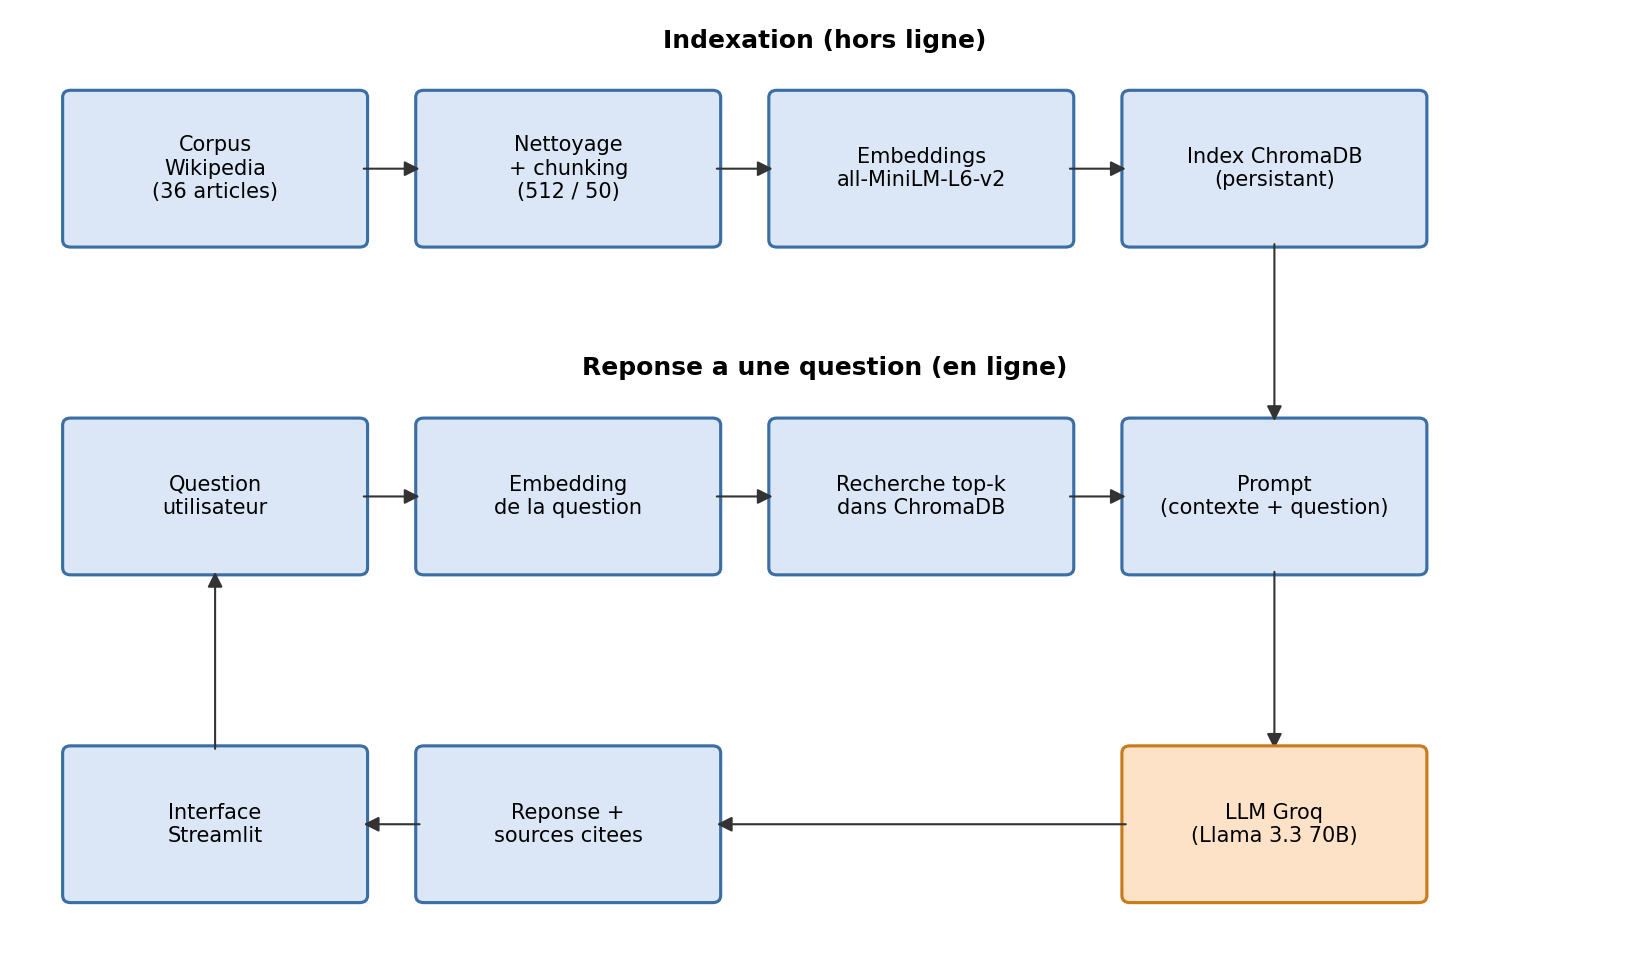
\includegraphics[width=\textwidth]{figures/architecture.png}
  \caption{Architecture g\'en\'erale du pipeline RAG (indexation hors ligne et r\'eponse en ligne).}
  \label{fig:archi}
\end{figure}

\subsection{Phase d'indexation (hors ligne)}

\begin{enumerate}[noitemsep]
  \item \textbf{Corpus} : 36 articles Wikipedia t\'el\'echarg\'es par \texttt{collect\_corpus.py}.
  \item \textbf{Nettoyage et chunking} : suppression des pages d'homonymie et des sections
        non informatives, puis d\'ecoupage en chunks de 512 caract\`eres avec un chevauchement
        de 50 caract\`eres (\texttt{src/prepare\_data.py}).
  \item \textbf{Embeddings} : chaque chunk est vectoris\'e avec \texttt{all-MiniLM-L6-v2}
        (\texttt{sentence-transformers}).
  \item \textbf{Index vectoriel} : vecteurs, textes et m\'etadonn\'ees (document source) stock\'es
        dans une collection ChromaDB persistante (\texttt{src/build\_index.py}).
\end{enumerate}

\subsection{Phase de r\'eponse (en ligne)}

\begin{enumerate}[noitemsep]
  \item La question utilisateur est encod\'ee avec le m\^eme mod\`ele d'embedding.
  \item ChromaDB renvoie les \texttt{top-3} chunks les plus proches (similarit\'e cosinus).
  \item Ces chunks sont ins\'er\'es dans un template de prompt avec la question.
  \item Le prompt est envoy\'e au LLM via l'API Groq (\texttt{llama-3.3-70b-versatile}).
  \item La r\'eponse et les sources sont affich\'ees dans le CLI ou l'interface Streamlit.
\end{enumerate}

\subsection{Organisation du d\'ep\^ot}

Le code source est versionn\'e sur GitHub :
\url{https://github.com/Muhammed-OTP/rag-nlp-m1}. Les param\`etres partag\'es (taille de chunk,
chevauchement, mod\`ele d'embedding, \texttt{top\_k}, mod\`ele Groq) sont centralis\'es dans
\texttt{config.py} pour \'eviter toute duplication.
